\documentclass[a4paper,french, titlepage]{article}

\usepackage[utf8]{inputenc}   % accents
\usepackage[T1]{fontenc}      % caractères français
\usepackage[french]{babel}    % langue
\usepackage[top=20mm, bottom=20mm, left=20mm , right=20mm]{geometry}		  % package marges
\usepackage{graphicx}         % images
\usepackage[graphicx]{realboxes}
\usepackage{verbatim}         % texte préformaté
\usepackage{moreverb}
\usepackage{amsmath,amsfonts,amssymb,amsthm}
\usepackage[all]{xy}		  % diagrammes
\usepackage{float} 			  % images
\usepackage{lscape}			  % pages paysage
\usepackage{url}			  % bibliographie
\usepackage{xcolor}			  % couleurs
\usepackage{verbatim, textcomp, fancyvrb,multicol} % programmes
\usepackage{framed}								   % programmes je crois
\usepackage{listings} % code java en couleurs
\usepackage{subfig}
%\usepackage{subfigure}
\usepackage{wrapfig}
\usepackage{mathrsfs}
\usepackage{amsmath}
\usepackage{hyperref}
\hypersetup{
    colorlinks = true,
    allcolors = {black}
}




% Personnalisation entêtes et pieds de pages
%\usepackage{mathpazo} % nouvelle police 
%\usepackage{fancyhdr}
%\pagestyle{fancy}

% Entêtes
%\renewcommand{\headrulewidth}{1pt}
%\fancyhead[C]{} 
%\fancyhead[L]{TER}
%\fancyhead[R]{Commande d'une ligne transitique MONTRAC}
%\headheight=1.1cm

% Pieds de pages
%\renewcommand{\footrulewidth}{1pt}
%\fancyfoot[C]{Bruno \bsc{Dato}, Abdellah \bsc{Elgourain} et Evgeny \bsc{Shulga}} 
%\fancyfoot[L]{M1 EEA / ISTR}
%\fancyfoot[R]{\thepage}

\title{{\Huge STAGE}\\Intégration et commande sous ROS du robot Baxter au sein d’une cellule flexible d’assemblage\\}
\author{Bruno \bsc{Dato}}
\date{30 juin 2016}


\begin{document}
 
%\maketitle  %page de garde
\thispagestyle{empty}

\begin{center}
Master 1 Électronique Électrotechnique Automatique, Ingénierie des Sytèmes Temps-Réel  
\vspace{0.5cm}

\begin{figure}[H] 
\begin{center}

\includegraphics[scale=0.3]{Images/logo_ups.jpg} 
\end{center}
\end{figure}





\vspace{0.3cm}

{\Huge STAGE}\\

\vspace{0.3cm}

{\Huge Intégration et commande sous ROS du robot Baxter au sein d’une cellule flexible d’assemblage}\\

\vspace{0.5cm}

\begin{figure}[H] 
\begin{center}
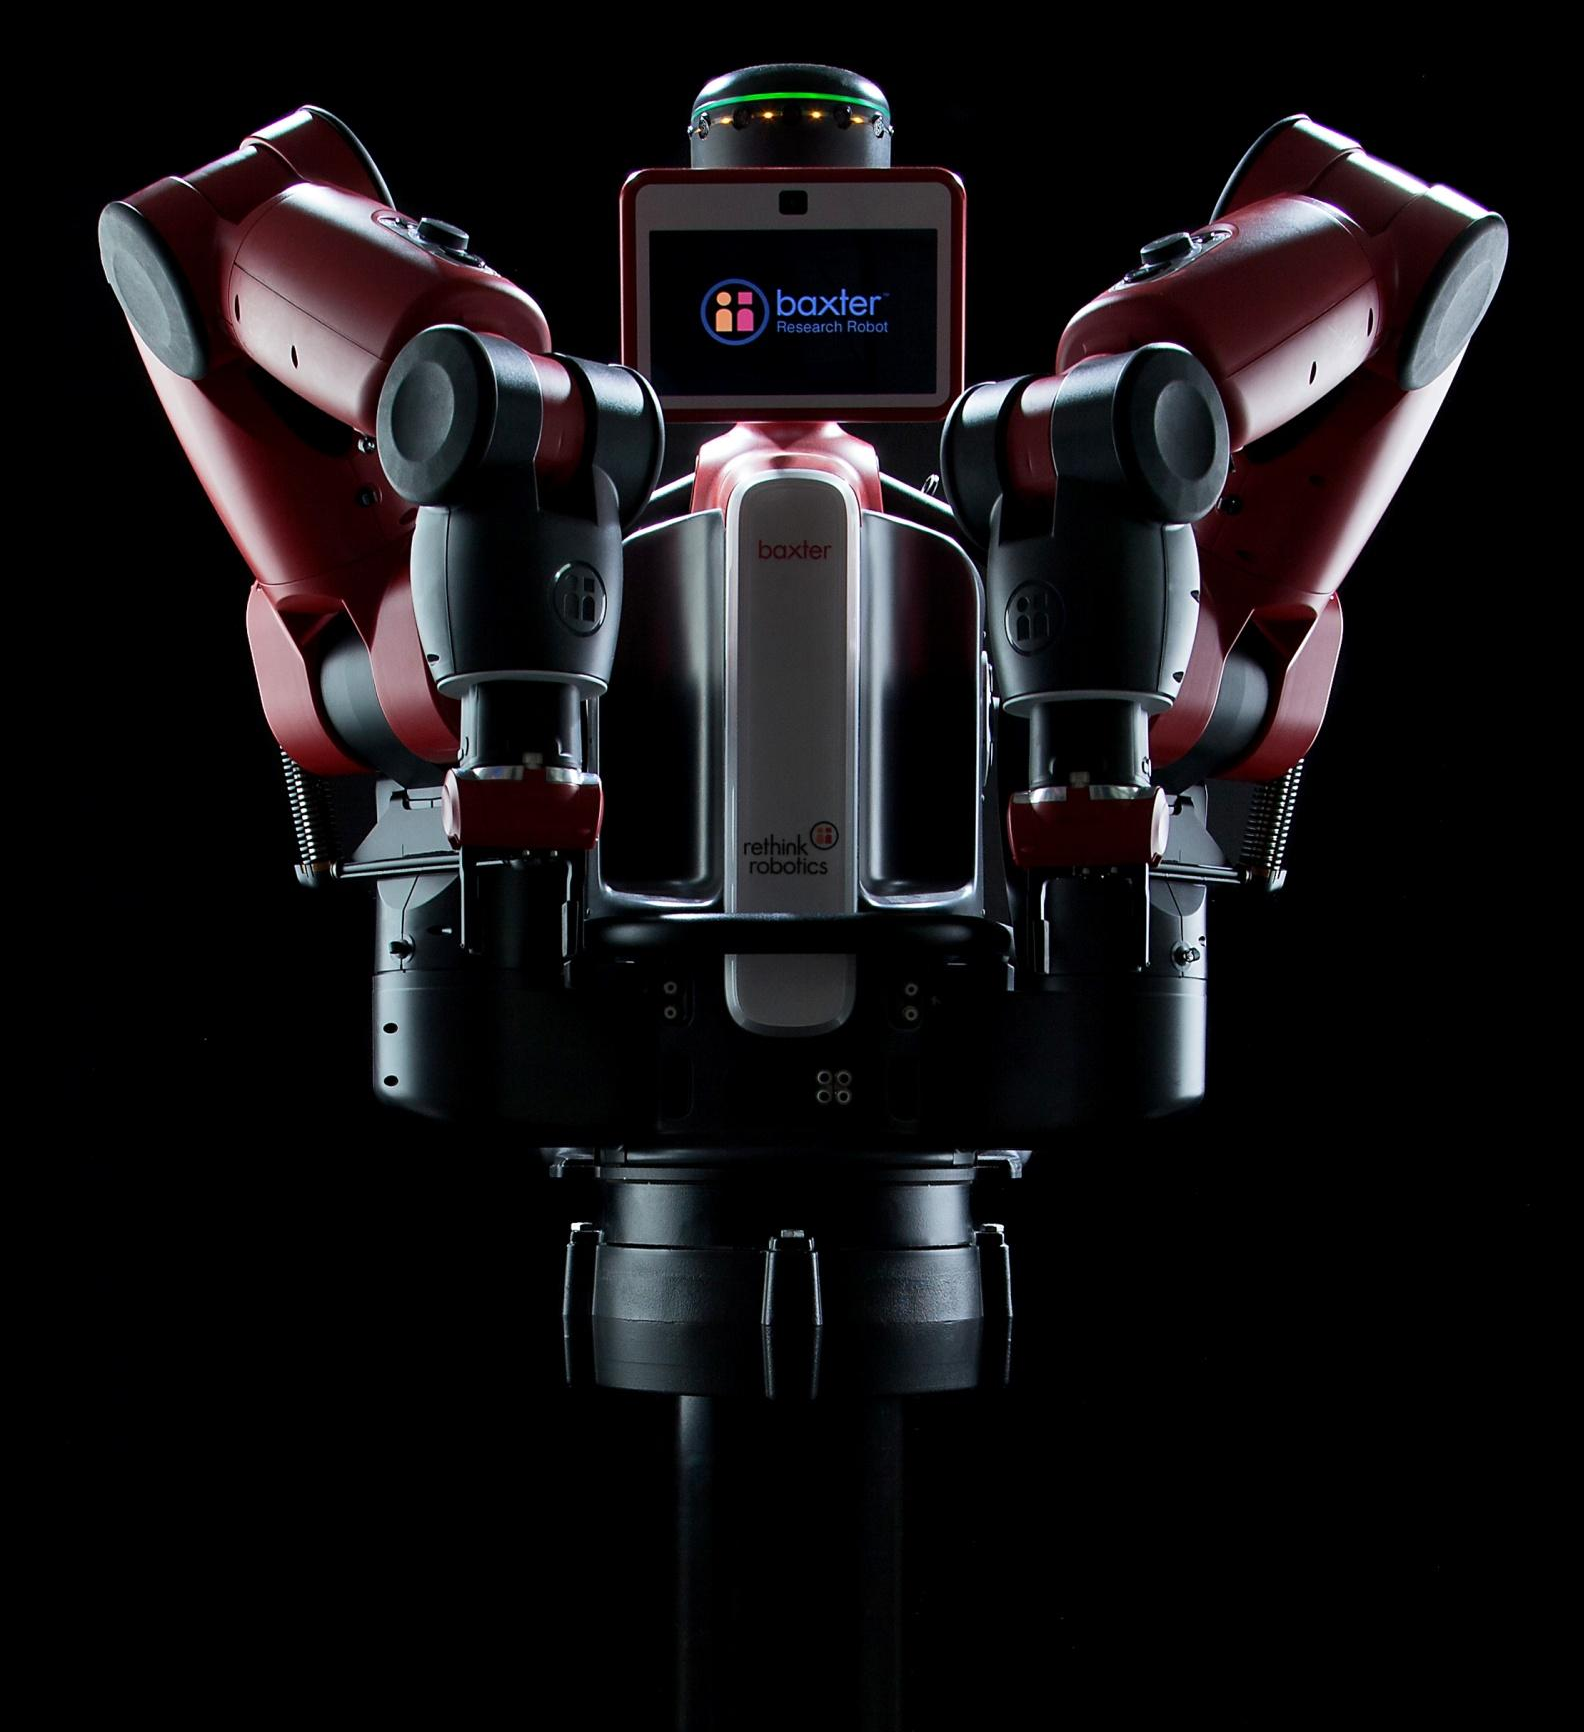
\includegraphics[scale=0.2]{Images/baxter.png}
\end{center}
\end{figure}

\vspace{0.5cm}

{\LARGE Auteur}\\

\vspace{0.2cm}

Bruno \bsc{Dato}\\

\vspace{0.5cm}

{\Large Encadrants}\\

\vspace{0.2cm}

C. Briand, M. Taïx\\ 



\vspace{1cm}


30 juin 2016




\end{center}

\newpage
\addcontentsline{toc}{section}{Remerciements}
\section*{Remerciements}

\vspace{5cm}

Je tiens à remercier mes encadrants de stage C. Briand et M. Taïx pour m'avoir permis de réaliser ce stage. Je remercie aussi toutes les personnes de l'AIP pour leur accueil au sein de la halle technologique durant toute la durée de mon stage.

\newpage
\renewcommand{\contentsname}{Sommaire} % permet de changer le titre de la table des matières
\tableofcontents %sommaire


\newpage
\addcontentsline{toc}{section}{Introduction}
\section*{Introduction}


\newpage
\section{Présentation du stage}

\subsection{Projet global}

\begin{figure}[H] 
\begin{center}
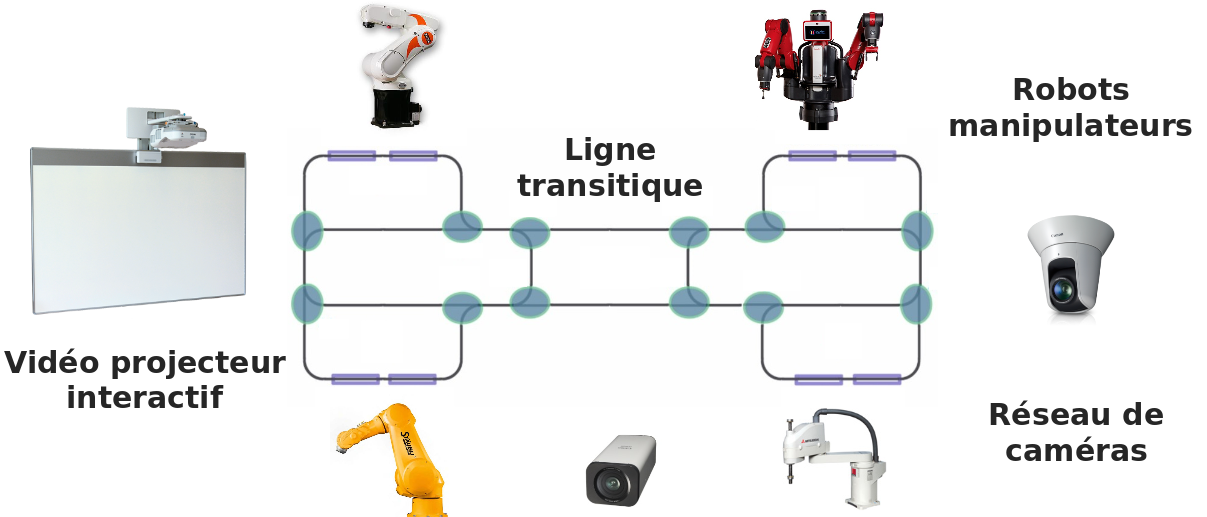
\includegraphics[scale=0.35]{Images/projet_global.png} 
\end{center}
\caption{Vue globale des systèmes à faire interagir dans un futur proche}
\label{projet_global}
\end{figure} 

\subsection{Le robot Baxter}


\begin{figure}[H] 
\begin{center}
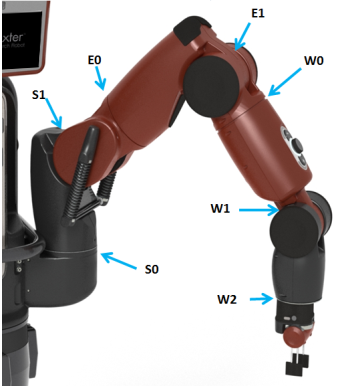
\includegraphics[scale=0.7]{Images/Baxter_arm.png} 
\end{center}
\caption{Les différents angles des bras du robot Baxter}
\label{Baxter_arm}
\end{figure} 


\newpage
\section{ROS}

\subsection{Les topics de Baxter}


\subsection{Les topics supplémentaires}


\subsection{Le noeud Commande$\_$Baxter}


\subsubsection{La classe Baxter}

\subsubsection{Les classes Baxter$\_$left$\_$arm et Baxter$\_$right$\_$arm}


\subsection{Le noeud Commande}

\subsubsection{La classe Communication$\_$Baxter}







\newpage
\section{Synthèse de commande}

\subsection{Commande du robot seul}

\begin{figure}[H] 
\begin{center}
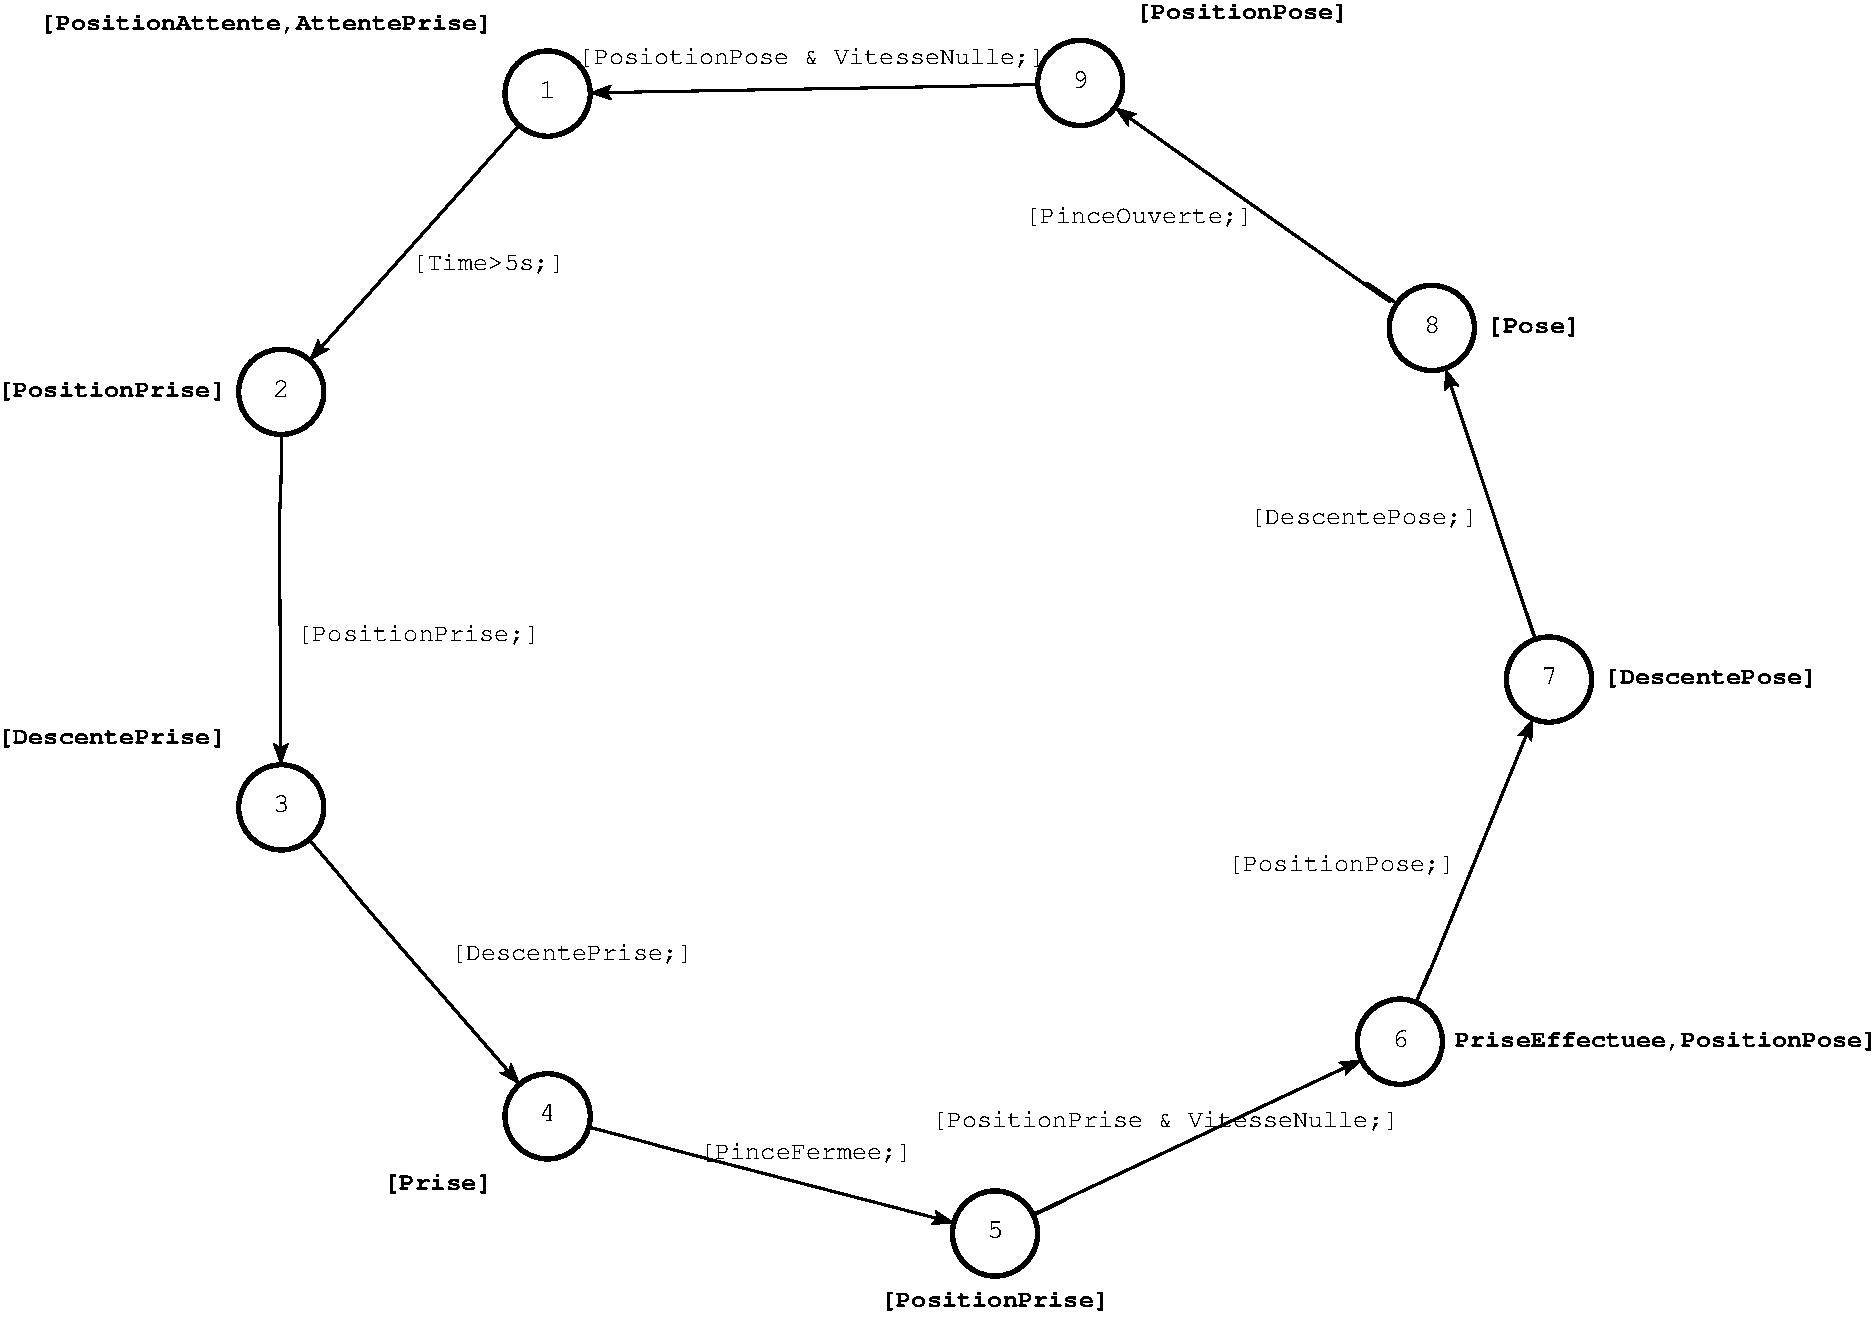
\includegraphics[scale=0.5]{Images/main_commande_1_bras.pdf} 
\end{center}
\caption{Machine à états finis de la commande d'un bras du robot Baxter}
\label{main_commande_1_bras}
\end{figure} 

\subsection{Commande de la ligne transitique MONTRAC en intération avec le robot Baxter}

\begin{figure}[H] 
\begin{center}
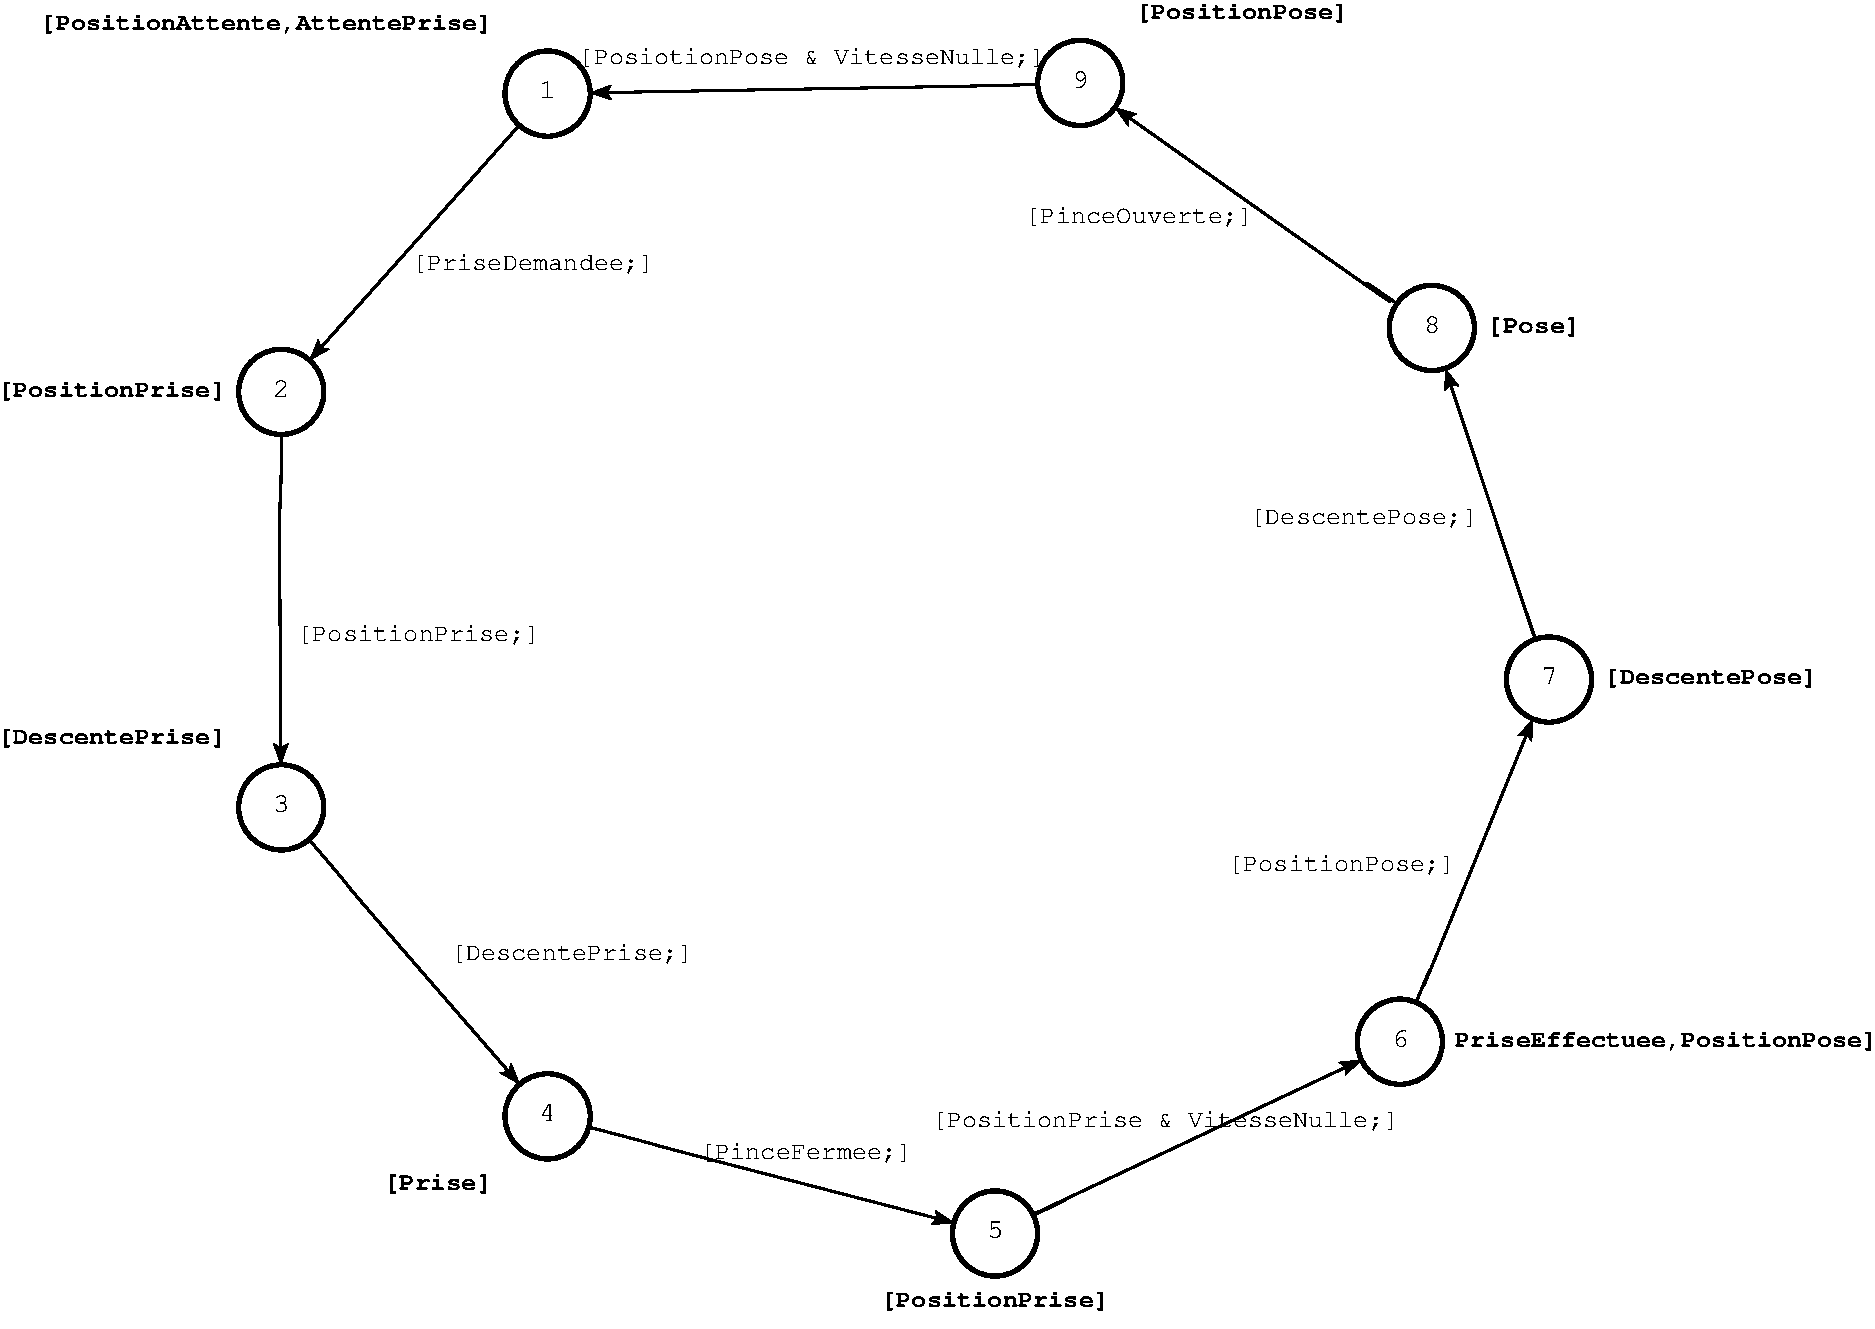
\includegraphics[scale=0.5]{Images/main_commande_bras_GD.pdf} 
\end{center}
\caption{Machine à états finis de la commande de chaqu'un des deux bras en interaction avec la ligne transitique}
\label{main_commande_bras_GD}
\end{figure}

\subsubsection{Commande de la ligne transitique en interaction avec un des bras manipulateurs}

 

\begin{figure}[H] 
\begin{center}
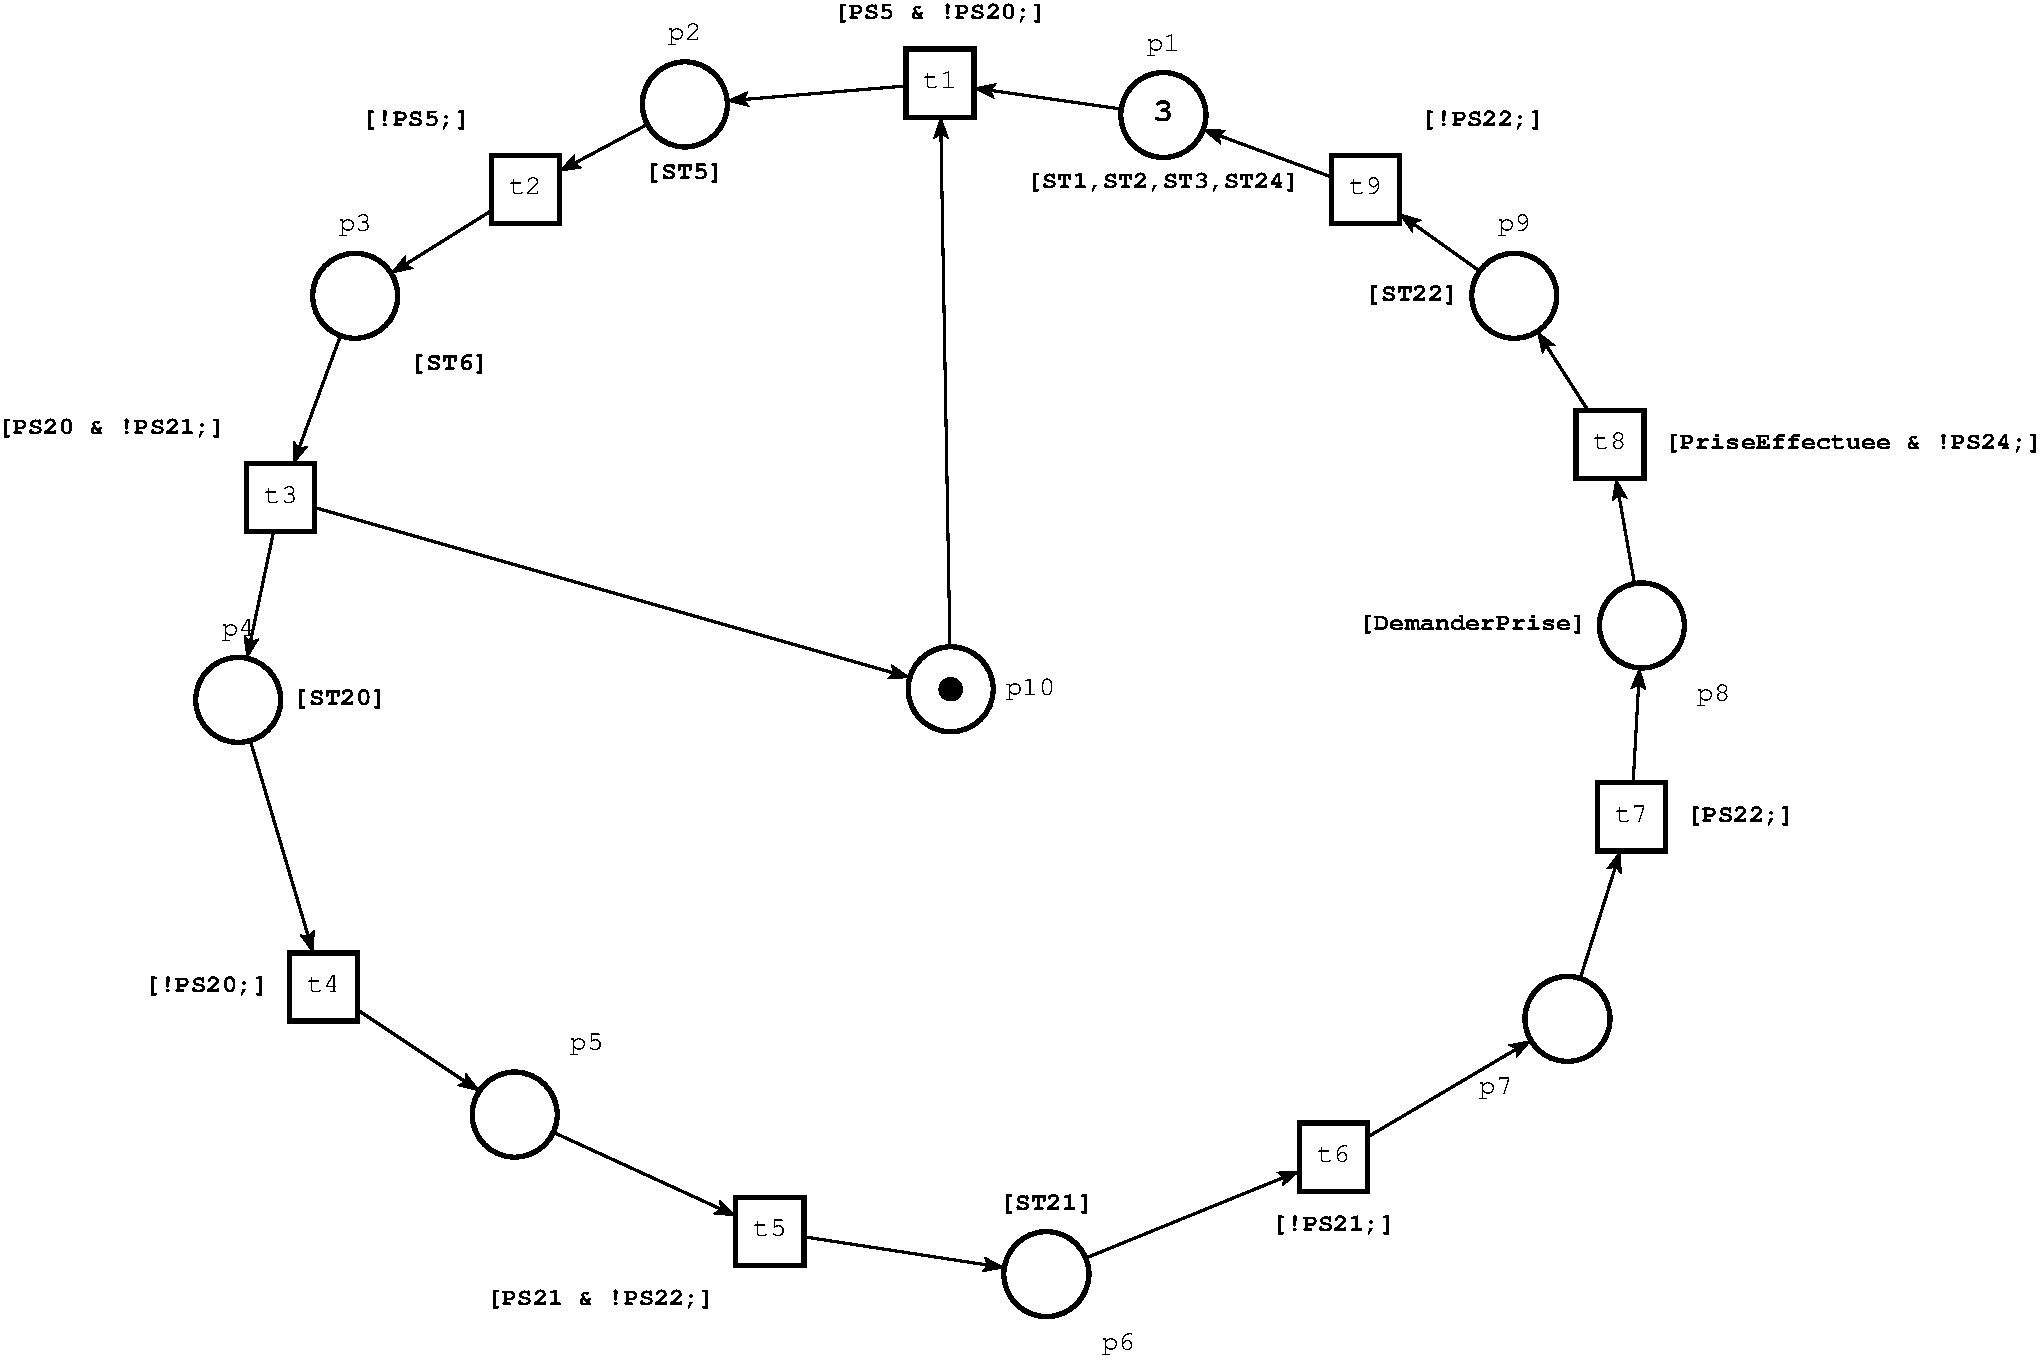
\includegraphics[scale=0.5]{Images/main_commande_baxter_1_bras_ligne_transitique.pdf} 
\end{center}
\caption{Réseau de Petri de la commande de la ligne transitique en interaction avec un bras du robot Baxter}
\label{main_commande_baxter_1_bras_ligne_transitique}
\end{figure}

\subsubsection{Commande de la ligne transitique en interaction avec les deux bras manipulateurs}


\begin{figure}[H] 
\begin{center}
\Rotatebox{90}{
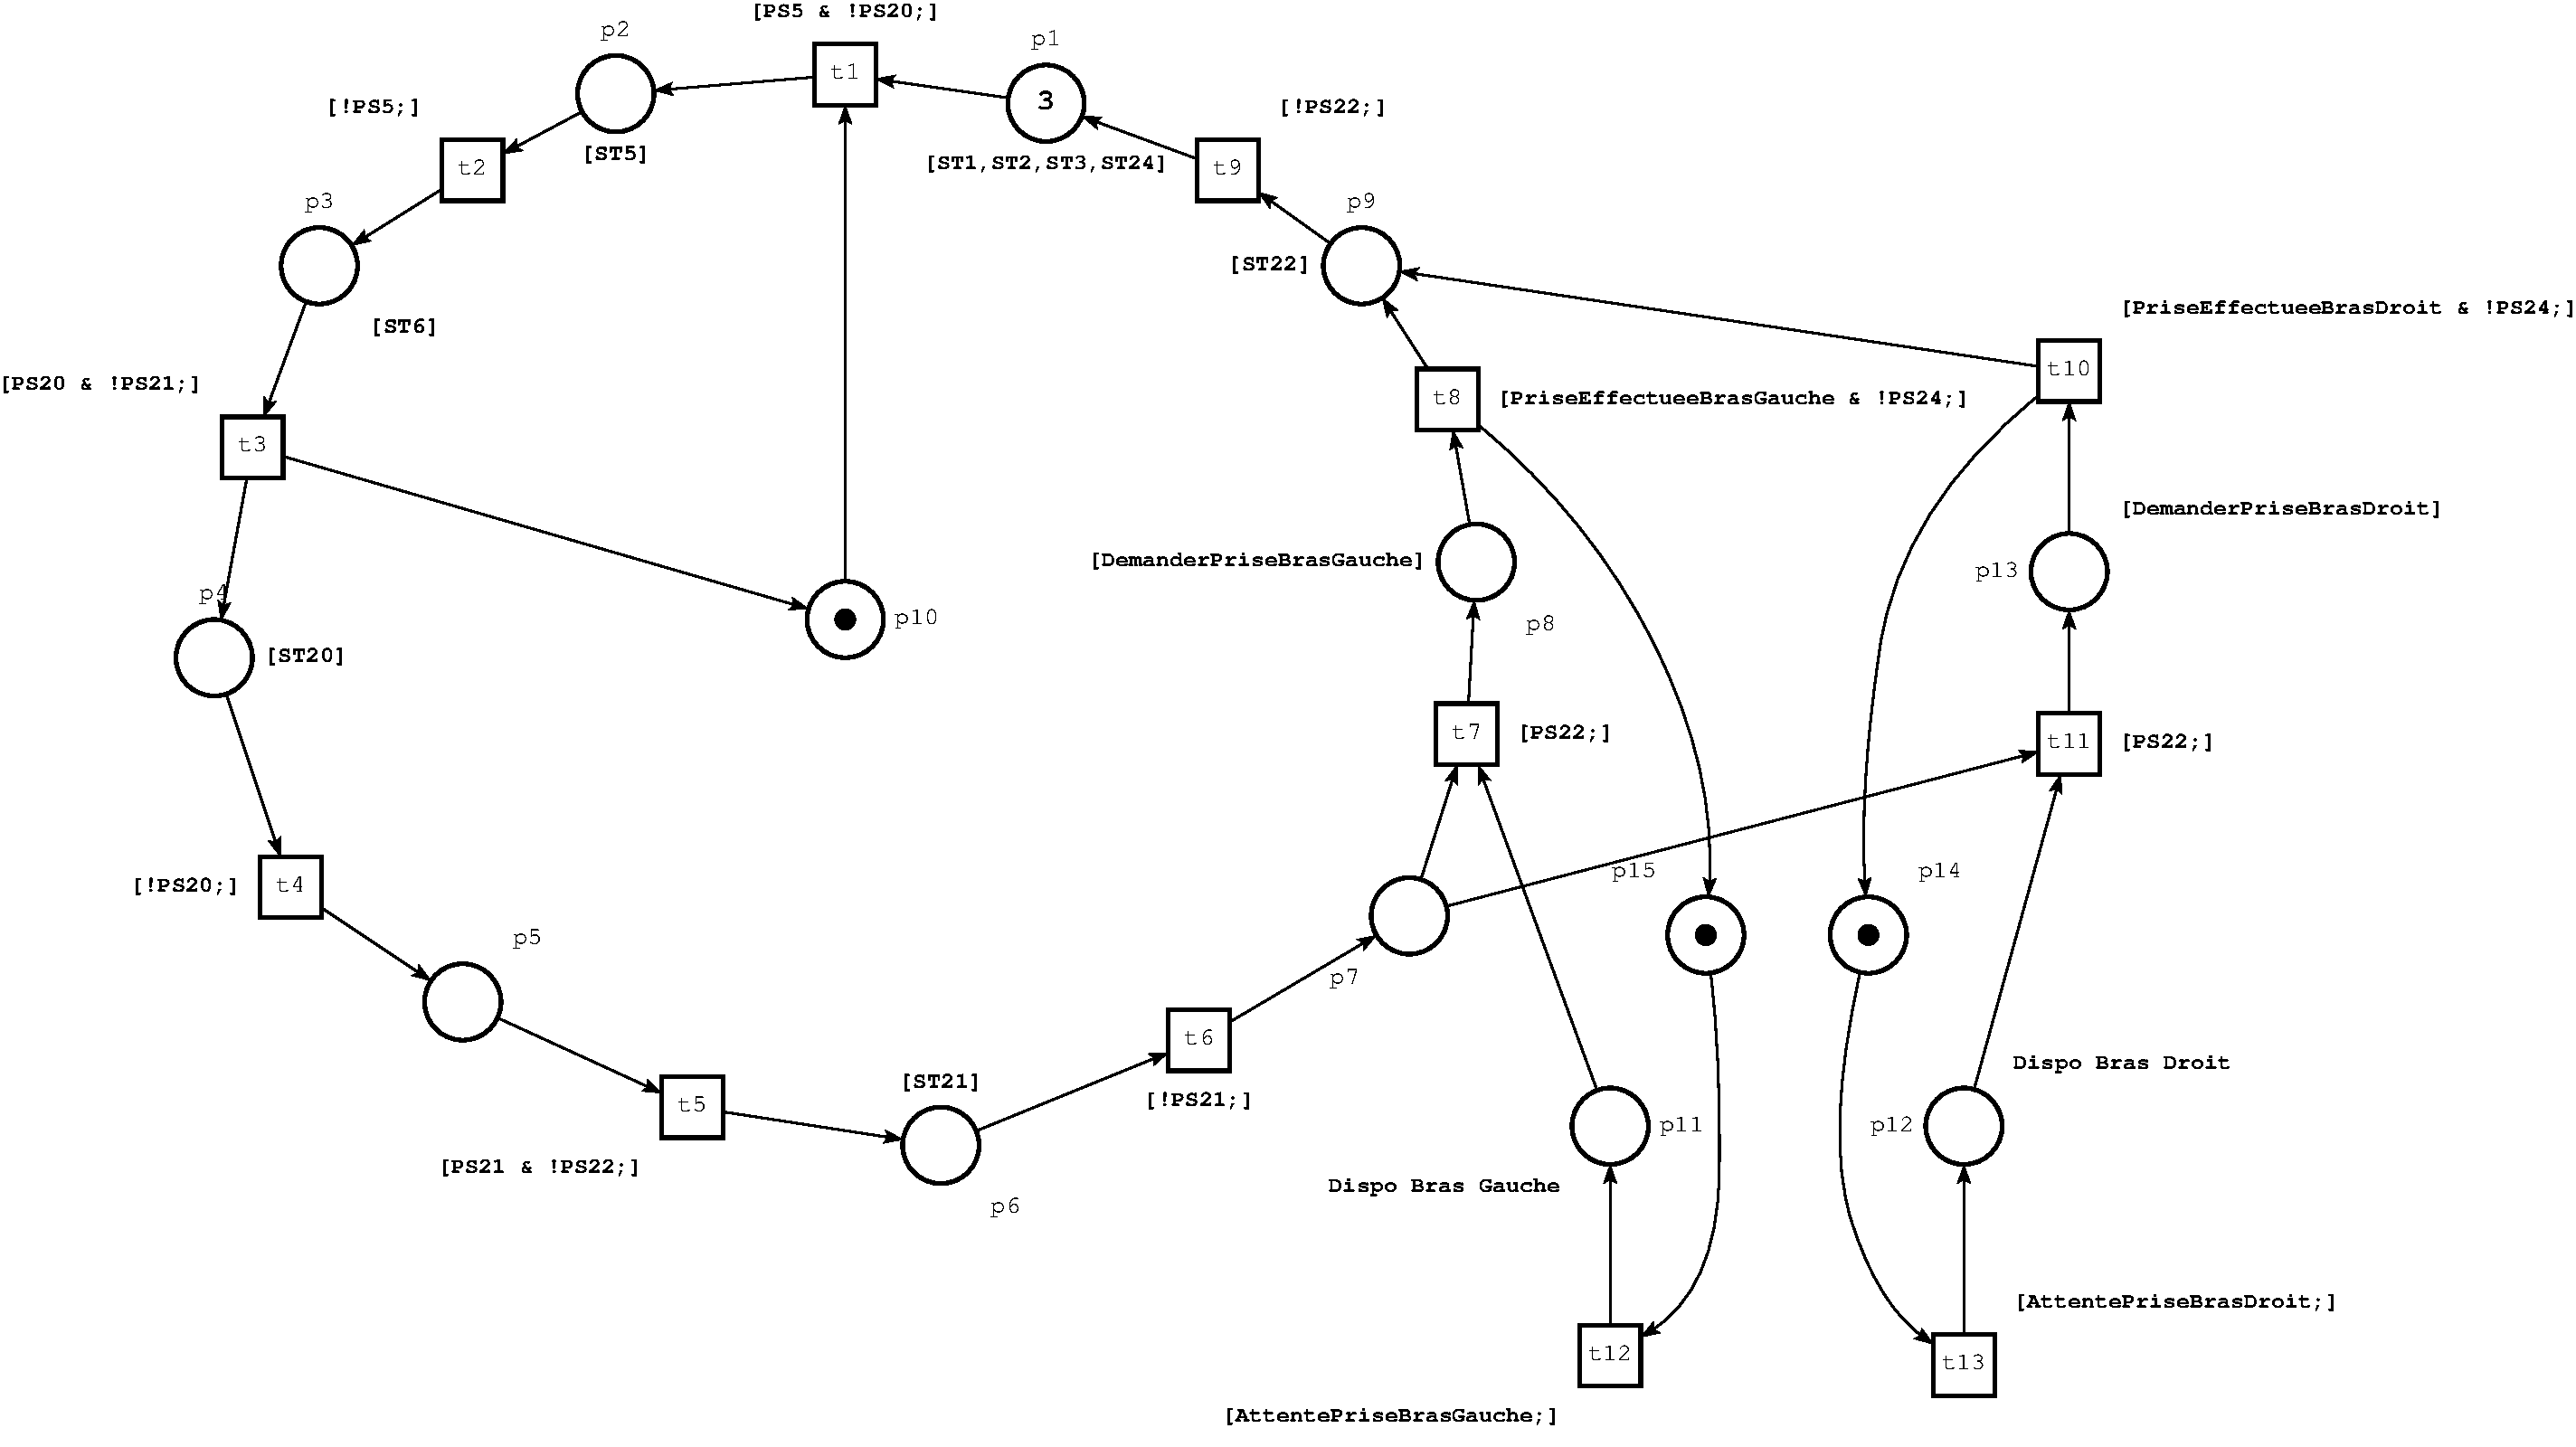
\includegraphics[scale=0.45]{Images/main_commande_baxter_2_bras_ligne_transitique.pdf} 
}
\end{center}
\caption{Réseau de Petri de la commande de la ligne transitique en interaction avec les deux bras du robot Baxter}
\label{main_commande_baxter_2_bras_ligne_transitique}
\end{figure}


\newpage
\addcontentsline{toc}{section}{Conclusion}
\section*{Conclusion}


\end{document}



